\documentclass[12pt]{article}

% Import this into main.tex doc with 
% Import this into main.tex doc with 
% Import this into main.tex doc with \input{preamble} after class definition
\usepackage[utf8]{inputenc}
% MATH
\usepackage{amsmath}
\usepackage{amssymb}
\usepackage{graphicx}
\usepackage{mathrsfs}
\usepackage{commath}
% [physics] contains nice derivative commands
\usepackage{physics}
% [bbold] contains doublestroke characters but overwrites several commands like \mathbb
% \usepackage{bbold}
% [cancel] allows the \cancelto{0}{x} command
\usepackage{cancel}
% adjusts height of the '\\' command for line breaks
\setlength{\jot}{10pt}


% FORMATTING
% this adjusts margins
% new margins for all pages
%\usepackage[bottom=.6in,top=.6in]{geometry}
% \newgeometry and \restoregeometry for page specific margins
\usepackage{geometry}
\usepackage[titletoc]{appendix}
\usepackage{caption}
\usepackage{float}
\usepackage{titling}
% [lscape] for making landscape pages \begin{landscape}
\usepackage{lscape}
% for subfigures (better than minipages)
% EX: \begin{subfigure}[t]{0.45\textwidth}
\usepackage{subcaption}
% for fancy tables
\usepackage{ragged2e}
\usepackage{array}
% define new column types for tabular environments
% these wrap text but you have to specify column width
% ex: \begin{tabular}{|L{4cm}|L{2cm}}
\newcolumntype{L}[1]{>{\raggedright\let\newline\\\arraybackslash\hspace{0pt}}m{#1}}
\newcolumntype{C}[1]{>{\centering\let\newline\\\arraybackslash\hspace{0pt}}m{#1}}
\newcolumntype{R}[1]{>{\raggedleft\let\newline\\\arraybackslash\hspace{0pt}}m{#1}}
% for inserting PDFs selectively
\usepackage{pdfpages}

% making hyperlinks throughout the document
\usepackage[linktocpage=true, breaklinks=true]{hyperref}
\hypersetup{
    colorlinks,
    citecolor=blue,
    filecolor=blue,
    linkcolor=blue,
    urlcolor=blue
}
\usepackage{lmodern}  % for bold teletype font
\usepackage{xcolor}   % for \textcolor
% lstlisting environment settings
\usepackage{listings}
\lstset{
  basicstyle=\ttfamily,
  columns=fullflexible,
  frame=single,
  breaklines=true,
  postbreak=\mbox{\textcolor{red}{$\hookrightarrow$}\space},
  showstringspaces=false,
  keepspaces=true,
  commentstyle=\color{gray},
  keywordstyle=\color{blue},
  stringstyle=\color{green},
  numbers=left
}

% changing name of abstract here
\renewcommand{\abstractname}{Yung Salad}

% SQUARE ROOT TAIL CODE

\usepackage{letltxmacro}
\makeatletter
\let\oldr@@t\r@@t
\def\r@@t#1#2{%
\setbox0=\hbox{$\oldr@@t#1{#2\,}$}\dimen0=\ht0
\advance\dimen0-0.4\ht0
\setbox2=\hbox{\vrule height\ht0 depth -\dimen0}%
{\box0\lower0.4pt\box2}}
\LetLtxMacro{\oldsqrt}{\sqrt}
\renewcommand*{\sqrt}[2][\ ]{\oldsqrt[#1]{#2}}
\makeatother
 after class definition
\usepackage[utf8]{inputenc}
% MATH
\usepackage{amsmath}
\usepackage{amssymb}
\usepackage{graphicx}
\usepackage{mathrsfs}
\usepackage{commath}
% [physics] contains nice derivative commands
\usepackage{physics}
% [bbold] contains doublestroke characters but overwrites several commands like \mathbb
% \usepackage{bbold}
% [cancel] allows the \cancelto{0}{x} command
\usepackage{cancel}
% adjusts height of the '\\' command for line breaks
\setlength{\jot}{10pt}


% FORMATTING
% this adjusts margins
% new margins for all pages
%\usepackage[bottom=.6in,top=.6in]{geometry}
% \newgeometry and \restoregeometry for page specific margins
\usepackage{geometry}
\usepackage[titletoc]{appendix}
\usepackage{caption}
\usepackage{float}
\usepackage{titling}
% [lscape] for making landscape pages \begin{landscape}
\usepackage{lscape}
% for subfigures (better than minipages)
% EX: \begin{subfigure}[t]{0.45\textwidth}
\usepackage{subcaption}
% for fancy tables
\usepackage{ragged2e}
\usepackage{array}
% define new column types for tabular environments
% these wrap text but you have to specify column width
% ex: \begin{tabular}{|L{4cm}|L{2cm}}
\newcolumntype{L}[1]{>{\raggedright\let\newline\\\arraybackslash\hspace{0pt}}m{#1}}
\newcolumntype{C}[1]{>{\centering\let\newline\\\arraybackslash\hspace{0pt}}m{#1}}
\newcolumntype{R}[1]{>{\raggedleft\let\newline\\\arraybackslash\hspace{0pt}}m{#1}}
% for inserting PDFs selectively
\usepackage{pdfpages}

% making hyperlinks throughout the document
\usepackage[linktocpage=true, breaklinks=true]{hyperref}
\hypersetup{
    colorlinks,
    citecolor=blue,
    filecolor=blue,
    linkcolor=blue,
    urlcolor=blue
}
\usepackage{lmodern}  % for bold teletype font
\usepackage{xcolor}   % for \textcolor
% lstlisting environment settings
\usepackage{listings}
\lstset{
  basicstyle=\ttfamily,
  columns=fullflexible,
  frame=single,
  breaklines=true,
  postbreak=\mbox{\textcolor{red}{$\hookrightarrow$}\space},
  showstringspaces=false,
  keepspaces=true,
  commentstyle=\color{gray},
  keywordstyle=\color{blue},
  stringstyle=\color{green},
  numbers=left
}

% changing name of abstract here
\renewcommand{\abstractname}{Yung Salad}

% SQUARE ROOT TAIL CODE

\usepackage{letltxmacro}
\makeatletter
\let\oldr@@t\r@@t
\def\r@@t#1#2{%
\setbox0=\hbox{$\oldr@@t#1{#2\,}$}\dimen0=\ht0
\advance\dimen0-0.4\ht0
\setbox2=\hbox{\vrule height\ht0 depth -\dimen0}%
{\box0\lower0.4pt\box2}}
\LetLtxMacro{\oldsqrt}{\sqrt}
\renewcommand*{\sqrt}[2][\ ]{\oldsqrt[#1]{#2}}
\makeatother
 after class definition
\usepackage[utf8]{inputenc}
% MATH
\usepackage{amsmath}
\usepackage{amssymb}
\usepackage{graphicx}
\usepackage{mathrsfs}
\usepackage{commath}
% [physics] contains nice derivative commands
\usepackage{physics}
% [bbold] contains doublestroke characters but overwrites several commands like \mathbb
% \usepackage{bbold}
% [cancel] allows the \cancelto{0}{x} command
\usepackage{cancel}
% adjusts height of the '\\' command for line breaks
\setlength{\jot}{10pt}


% FORMATTING
% this adjusts margins
% new margins for all pages
%\usepackage[bottom=.6in,top=.6in]{geometry}
% \newgeometry and \restoregeometry for page specific margins
\usepackage{geometry}
\usepackage[titletoc]{appendix}
\usepackage{caption}
\usepackage{float}
\usepackage{titling}
% [lscape] for making landscape pages \begin{landscape}
\usepackage{lscape}
% for subfigures (better than minipages)
% EX: \begin{subfigure}[t]{0.45\textwidth}
\usepackage{subcaption}
% for fancy tables
\usepackage{ragged2e}
\usepackage{array}
% define new column types for tabular environments
% these wrap text but you have to specify column width
% ex: \begin{tabular}{|L{4cm}|L{2cm}}
\newcolumntype{L}[1]{>{\raggedright\let\newline\\\arraybackslash\hspace{0pt}}m{#1}}
\newcolumntype{C}[1]{>{\centering\let\newline\\\arraybackslash\hspace{0pt}}m{#1}}
\newcolumntype{R}[1]{>{\raggedleft\let\newline\\\arraybackslash\hspace{0pt}}m{#1}}
% for inserting PDFs selectively
\usepackage{pdfpages}

% making hyperlinks throughout the document
\usepackage[linktocpage=true, breaklinks=true]{hyperref}
\hypersetup{
    colorlinks,
    citecolor=blue,
    filecolor=blue,
    linkcolor=blue,
    urlcolor=blue
}
\usepackage{lmodern}  % for bold teletype font
\usepackage{xcolor}   % for \textcolor
% lstlisting environment settings
\usepackage{listings}
\lstset{
  basicstyle=\ttfamily,
  columns=fullflexible,
  frame=single,
  breaklines=true,
  postbreak=\mbox{\textcolor{red}{$\hookrightarrow$}\space},
  showstringspaces=false,
  keepspaces=true,
  commentstyle=\color{gray},
  keywordstyle=\color{blue},
  stringstyle=\color{green},
  numbers=left
}

% changing name of abstract here
\renewcommand{\abstractname}{Yung Salad}

% SQUARE ROOT TAIL CODE

\usepackage{letltxmacro}
\makeatletter
\let\oldr@@t\r@@t
\def\r@@t#1#2{%
\setbox0=\hbox{$\oldr@@t#1{#2\,}$}\dimen0=\ht0
\advance\dimen0-0.4\ht0
\setbox2=\hbox{\vrule height\ht0 depth -\dimen0}%
{\box0\lower0.4pt\box2}}
\LetLtxMacro{\oldsqrt}{\sqrt}
\renewcommand*{\sqrt}[2][\ ]{\oldsqrt[#1]{#2}}
\makeatother


\title{Robotics Prototyping Package Math and Algorithms}
\author{Ben Kolligs}
\date{}

\begin{document}
	\maketitle
	\tableofcontents
	\break
	\section{Core Classes}
	\subsection{Transform}
	The main class of the core of the package is the Transform class. 
	This class performs the functionality of a homogeneous rigid transform, which shows up in many places within robotics and robotics adjacent fields, like computer vision and graphics. 

	% The transform document describing the transform class
	The homogeneous rigid transform is an extremely useful tool used to represent various things in robotics. 
First, the rigid transform is defined as a transformation $T$ that when acting on any vector $v$, produces a transformed vector $T(v)$ of the form: 
\begin{equation}
	T(v) = R v + t
\end{equation}

where $R^T R^{-1}$, and $t$ is a vector giving the translation of the origin. 
This concept can be represented in a form called a {\it homogeneous transformation matrix}. 
A homogeneous transformation matrix $T \in \mathbb{R}^{4 \times 4}$ is a member of special euclidean group $SE(3)$, and can be written in the form:
\begin{equation}
	T = \begin{bmatrix}
		R & t \\
		\bf{0} & 1
	\end{bmatrix}
\end{equation}
where $R \in \mathbb{R}^{3 \times 3}$ is a rotation matrix, and $t \in \mathbb{R}^3$ is a translation vector. 
The inverse of a homogeneous transformation matrix is:
\begin{align}
	T^{-1} &= 
	\begin{bmatrix}
		R^T & -R^Tt \\
		\bf{0} & 1
	\end{bmatrix} \\
	T T^{-1} &= \bf{I}
\end{align}
When using super and subscripts to specify the frames we are referring to, then $T_b^a = (T_a^b)^{-1}$.
We can use a homogeneous transformation to operate on homogeneous points $p, q \in \mathbb{R}^4$, 
\begin{align}
	q &= Tp \\
	\begin{bmatrix} 
		x_q \\ 
		y_q \\
		z_q \\
		1
	\end{bmatrix}
	&= \begin{bmatrix}
		R & t \\
		\bf{0} & 1
	\end{bmatrix} 
	\begin{bmatrix}
		x_p \\
		y_p \\
		z_p \\
		1
	\end{bmatrix}.
\end{align}

In general, there are three interpretations for homogeneous transformations:
\begin{enumerate}
	\item A description of relative orientation and translation between frames. 
	\item A coordinate transform between frames. 
	Specifically, $T_j^i$ is a transform from frame ${j}$ to frame ${i}$:
	\begin{equation}
		P^i = T_j^i P^j
	\end{equation}
	\item A motion of a point (or a collection of points) within a single frame. For example, as we saw above point $p$ can be moved to point $q$:
	\begin{align}
		q &= Tp \\
		P_2^i &= T_j^i P^i_1
	\end{align}
	Similarly, a homogeneous transform can represent a motion from one frame to another.
	Specifically, $T_j^i$ moves frame $i$ to frame $j$. 
\end{enumerate}
It is important to specify which of these interpretations you are using within your program, as it can get confusing what these transformations represent if people aren't on the same page. 

Additionally, one must pay attention to the frame that the operand is in, as this determines the function of the transform to some degree. 
$P_2^i = T^i_j P_1^i$ is a motion that operates on point $P_1^i$ within frame $i$ whereas $P^i = T_j^i P^j$ is a coordinate transformation from $j$ to $i$, and therefore if we feed a point in frame $j$ to this transformation, the point will not move, but the coordinates will be transformed into frame $i$, which is often desired.  

\subsection{Transforming between frames}
We can chain together homogeneous transforms to represent a traversal through frames. 
\begin{figure}[H]
	\centering
	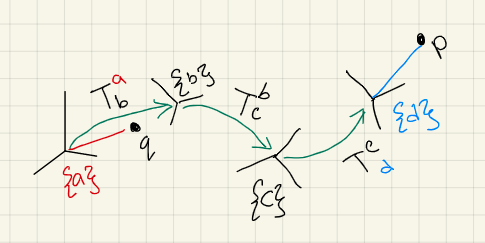
\includegraphics[width=0.8\textwidth]{images/frame_traversal.png}
	\caption{Traversing through different coordinate frames represented by rigid transformation matrices.}
	\label{fig: frames}
\end{figure}

Say we want the transform from $a$ to $d$:
\begin{equation}
	T_d^a = T^a_b T^b_c T^c_d.
\end{equation}
Notice that the bottom subscript and the following top subscript "cancel" out when multiplying frames together. 
Additionally when composing transforms like this, the "source" frame (in this case $d$) is included in the right most transform, and the "destination" frame $a$, is included in the left most. 

Using this knowledge we can represent frames that are related in this way by a pose graph, or pose tree consisting of parent and child relationships between each frame. 

\begin{figure}[H]
	\centering
	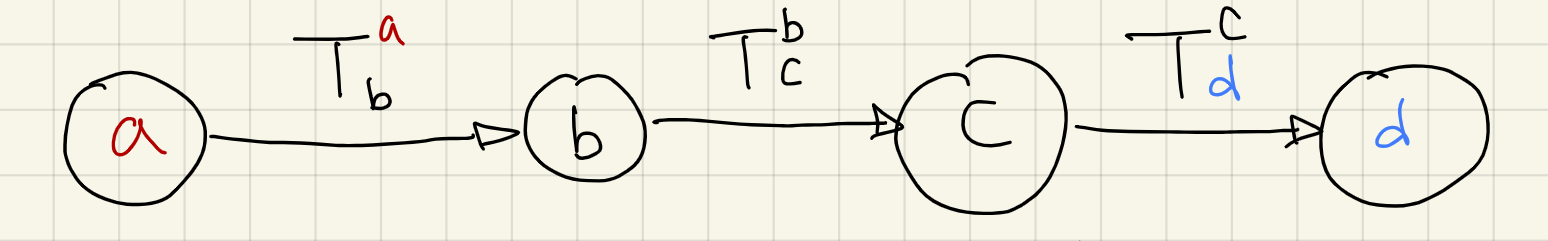
\includegraphics[width=0.8\textwidth]{images/pose_graph.png}
	\caption{Frames and their transforms can be represented in graph form.}
	\label{fig: poses}
\end{figure}
	\section{Pointcloud}
	The pointcloud class contains a list of 3D points in space. 
When transforming the entire pointcloud, the class simply creates homogeneous points out of the point list, and then multiplies a given homogeneous transform by this array. 
So if we want to transform the coordinates of pointcloud $C^i$ from frame $i$ into frame $j$:
\begin{equation}
	C^i = \begin{bmatrix}
		x_1 & x_2 & x_3 & \dots & x_n \\
		y_1 & y_2 & y_3 & \dots & y_n \\
		z_1 & z_2 & z_3 & \dots & z_n \\
		1 & 1 & 1 & \dots & 1
	\end{bmatrix}
\end{equation}

Then we need to multiply by the transform $T_i^j$: 
\begin{equation}
	C^j = T_i^j C^i.
\end{equation}

	\section{Rigid Collection}
	\label{sec: rigid}
	The rigid collection class $\cal{T}$ is simply a set of transforms, ${\cal T} = \{T_1, T_2, T_3, \dots T_n\}$.
It is required that this list of transforms be expressed in the same datum frame, that is:
\begin{equation}
	{\cal T}^i = \{T_1^i, T_2^i, T_3^i, \dots, T_n^i\}
\end{equation}
The rigid collection is able to be graphed in its "parent" frame $i$, which allows all contained transforms to be visualized. 
The collection is able to add transforms to itself by simply appending new transforms to the set. 

	\section{Kinematic Tree}
	\label{sec: kin tree}
	The kinematic tree is an abstract representation of a collection of transforms. 
Unlike the rigid collection (section \ref{sec: rigid}), the kinematic tree is able to represent transforms in multiple datum frames. 
The tree can then use the network of frames to "lookup" a transform between any two connected nodes, as hinted at in figure \ref{fig: poses}.
This concept is widely used in robotics and therefore has a place in the prototyping package. 
There are several algorithms this class implements:
\begin{enumerate}
	\item Representation: Construct a tree representation given only the edges
	\item Lookup: apply breadth first graph search to find a path between any two nodes on the tree
	\item Root: use depth first search to express all frames in the base link frame or another specified frame on the tree
\end{enumerate}

\subsection{Representation}
Frames in a kinematic tree must have a child frame, a parent frame, or both. 
Frame $T$ is described as:
\begin{equation}
	T_i^{p(i)} = \begin{bmatrix}
		R_i^{p(i)} & t_i^{p(i)} \\
		\bf{0} & 1
	\end{bmatrix}
\end{equation}
where $i$ is the child frame, and $p(i)$ is the parent frame. 
The kinematic tree has a root, which we can also call the "base link". 
The challenge with the kinematic tree is that we are only given the transforms, which are the edges in the graph. 
So we need to create a tree representation from just the transforms. 
Transforms contain the parent and child of the edge, and are therefore directed. 
Thus we want a representation that is easily able to express the directed nature of the graph. 

The importance of the edges in the kinematic tree suggests that an incidence list is the best representation for this situation. 
For example, say we have a tree as shown in figure \ref{fig: tree}.

\begin{figure}
	\centering
	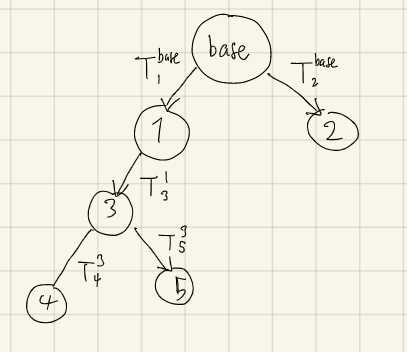
\includegraphics[width=0.5\textwidth]{images/example_tree.png}
	\caption{Example tree}
	\label{fig: tree}
\end{figure}

This takes the form:
\begin{align}
	base &: \big[ T^{base}_1, T^{base}_2\big] \\
	1 &: \big[ T^1_3, T^1_{base} \big]\\
	2 &: \big[ T^2_{base}\big]\\
	3 &: \big[ T_4^3, T_5^3 \big] \\
	4 &: \big[ T_3^4\big] \\
	5 &: \big[ T_3^5\big] \\
\end{align}
We can improve memory storage by using a dictionary (hash map) in order to only save the relevant edges. 
The construction algorithm is shown in algorithm \ref{alg: inc_list}.

\begin{algorithm}
	\DontPrintSemicolon
	\KwIn{Edge set $T$}
	\KwOut{Hash map where frames are the keys and the transforms they are incident with are values}
	tree $\gets \{\}$

	\tcp{hash.insert(key : value)}
	tree.insert(root : $\varnothing$)

	\For{$t \in T$}{$p \gets t.parent$

		$c \gets t.child$

		\tcp{process parents first}
		\If{$p \neq NULL$}{
			\eIf{$p \in$ tree}{
				\tcp{we store list of transforms touching $p$}
				tree[$p$].append($t$)
			}{
				tree.insert($p : \varnothing$)
			}
		}

		\tcp{process children}
		\If{$c \neq NULL$}{
			\eIf{$c \in $ tree}{
				\tcp{store whether the edge is forwards (used later)}
				($t^{-1}).forwards \gets false$

				tree[$c$].append($t^{-1}$)
			}{
				tree.insert($c : \varnothing$)
			}

		}
	}

	\Return{tree}
	\caption{Incidence list representation for the Kinematic Tree}
	\label{alg: inc_list}
\end{algorithm}

Once the incidence list is constructed, then we can use it to query the tree to find paths between frames.
The incidence list can keep track of the direction by assigning a flag to each edge specifying whether it is backwards or forwards. 
This will be useful for the rooting algorithm, shown later. 

\subsection{Lookup path between frames}

Now say we wanted to know the transform between two frames $i, j$ on the tree that aren't connected by an existing edge. 
We can find this edge, $T_i^j$ by finding the path between the two frames, and then multiplying the transforms we pass through. 

\begin{figure}
	\centering
	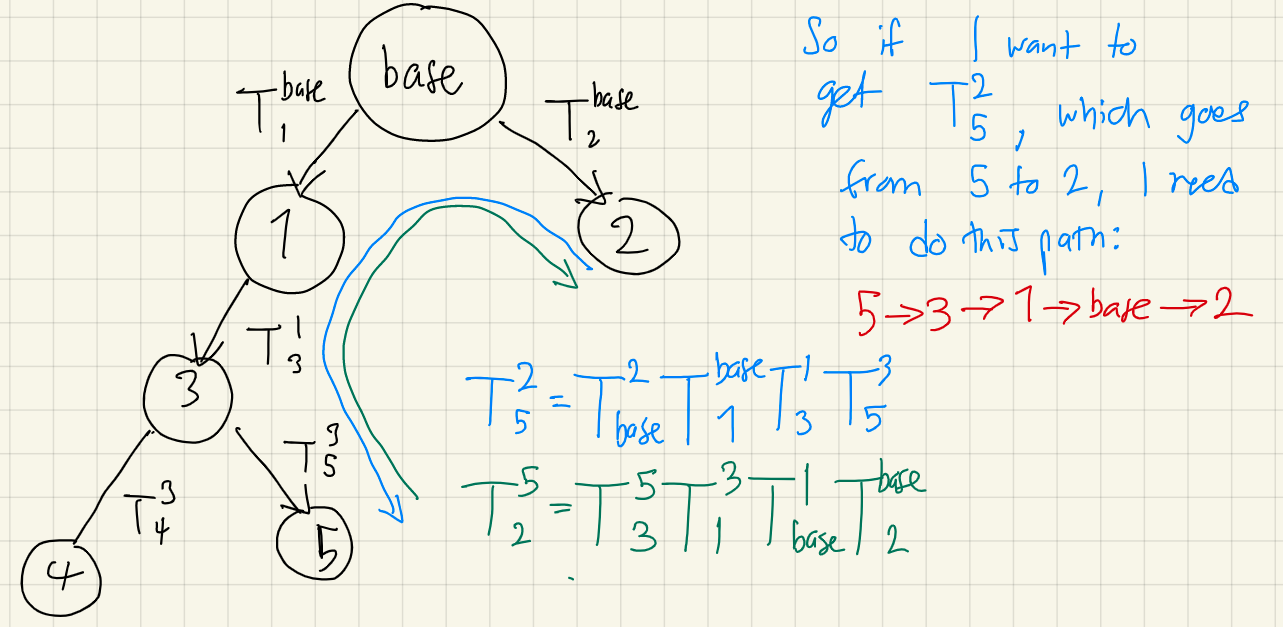
\includegraphics[width=\textwidth]{images/lookup_path.png}
	\caption{Lookup path between frames}
	\label{fig: lookup}
\end{figure}

\end{document}